%\documentclass[german,bachelor]{webisthesis}
\documentclass[english,bachelor]{webisthesis}
% When you change the language, pdflatex may halt on recompilation.
% Just hit enter to continue and recompile again. This should fix it.

%
% Values
% ------
\ThesisSetTitle{Authorship Verification with Phonetic Transcriptions}
\ThesisSetKeywords{Authorship Verification, Phonetic Transcription} % only for PDF meta attributes

\ThesisSetAuthor{David Reinartz}
\ThesisSetStudentNumber{3706997}
\ThesisSetDateOfBirth{2}{5}{1998}
\ThesisSetPlaceOfBirth{Ostercappeln}

\ThesisSetSupervisors{Prof.\ Dr.\ Martin Potthast,Prof.\ Dr.\ Benno Stein}

\ThesisSetSubmissionDate{31}{7}{2021}

%
% Suggested Packages
% ------------------
\usepackage[sort&compress]{natbib}
%   Allows citing in different ways (e.g., only the authors if you use the
%   citation again within a short time).
%
\usepackage{booktabs}
%    For tables ``looking the right way''.
%
\usepackage{tabularx}
%    Enables tables with columns that automatically fill the page width.
%
%\usepackage[ruled,algochapter]{algorithm2e}
%    A package for pseudo code algorithms.
%
\usepackage{amsmath}
%    For tabular-style formatting of mathematical environments.
%

%
% Commenting (by your supervisor)
% -------------------------------
\usepackage{xcolor}
\usepackage{soul}
\usepackage{amssymb}
\usepackage{svg}
%\setsvg{inkscape=inkscape -z -D,svgpath=figures/}
%\usepackage[clean]{svg}
\usepackage{tipa}
\usepackage{graphicx}
\newcommand{\bscom}[2]{%
  % #1 Original text.
  % #2 Replacement text.
    \st{\scriptsize\,#1}{\color{blue}\scriptsize\,#2}%
  }

% Create links in the pdf document
% Hyperref has some incompatibilities with other packages
% Some other packages must be loaded before, some after hyperref
% Additional options to the hyperref package can be provided in the braces []
\usehyperref[backref] % This will add back references in the bibliography

\begin{document}
\begin{frontmatter}
\begin{abstract}
% Short motivation / setting?
% Auth Ident. is ...
% Own task
% Results / contribution
\end{abstract}

  \tableofcontents

  %\chapter*{Acknowledgements} % optional
  %I thank the authors of the webisthesis template for their excellent work!

  %\listoffigures % optional

  %\listoftables % optional

  %\listofalgorithms % optional
  %    requires package algorithm2e

  % optional: list of symbols/notation (e.g., using the nomencl package)
\end{frontmatter}

\chapter{Introduction}\label{introduction}
With the widespread availability and use of text as a medium of information transfer, the problem of identifying authorship of given texts has become one of the main focuses of stylometric analysis.
In this paper, we specifically tackle the task of Authorship Verification which consists of classifying whether two given texts were written by the same author or not.
Underlying our approach is the hypothesis that authors have a \textit{phonetic preference}, based on which they produce different texts.
\cite{ladefoged2014courseInPhonetics} titles this preference the ``phonetics of the individual'' and states that ``[...] the set of phonetic habits and memories that each speaker possesses is different from those of every other speaker of the language''.
By applying phonetic transcription systems of varied granularity to the data used, we aim to emphasize these phonetically relevant features implanted into the texts by their authors.
Then, we use the transcribed data to train two well-known Authorship Verification classifiers.
By evaluating the results with standard measures used in Authorship Verification, we aim to answer the following questions:
\begin{itemize}
  \item Does the prior phonetic transcription of texts improve the performance of the algorithms over using verbatim text?
  \item Are the results correlated to the granularities of the transcriptions?
\end{itemize}
We transcribe textual data to North American English pronunciation.
We are aware that in this process some author-specific information is lost and will discuss the implications of this.
Nevertheless, we anticipate that the phonetic information encoded into plain text and boosted by transcribing gives the classifiers an advantage over more na\"{\i}ve methods.
All code attributions are open-sourced at \url{https://github.com/torond/bachelors-thesis} with an emphasis on ease of reproduction.


% % Showing natbib citation commands
% Let us get started by citing \citet{manning:1999}!
% So what did \citeauthor{manning:1999} do in % \citeyear{manning:1999}?
% Good question!
% % Showing hyperref reference commands
% Maybe it is answered in \autoref{introduction} on % page~\pageref{introduction}?
% Just to have something show up in the list of figures, I % included \autoref{fig:a}.
% \begin{figure}[bt]% bottom or top of page (for small % figures/tables)
%   \begin{center}{\huge\bf A}\end{center}
%   \caption{The first letter in the Roman % alphabet.}\label{fig:a}
% \end{figure}
% % \formatdate (or \formatdateshort)
% This date does not exist: \formatdateshort{30}{2}{2014}
% and is the same as \formatdate{30}{2}{2014}.
% % An example table
% And here is some table with some numbers % (\autoref{tab:numbers})
% which deserves to be on an extra page.
% \begin{table}[p]% extra page (usually for large figures/tables)
%   \caption{Tables have their captions above, figures below.}
%   \begin{center}
%     \begin{tabular}{lccc}\toprule
%       \multicolumn{4}{c}{Some numbers}\\\midrule
%       & 1999 & 2000 & 2001 \\\cmidrule(l){2-4}
%       % cmidrule: A line from 2nd to 4th column, trimmed on the % left hand side
%       Distance (km) & 23 & 18 & 42 \\
%       Awesomeness (aws) & 3.2 & 8.1 & 2.4 \\\bottomrule
%     \end{tabular}
%   \end{center}\label{tab:numbers}%
% \end{table}
\chapter{Background}\label{ch:background}
% Authorship Verification
\section{Authorship Verification}\label{sec:authorship-verification}
In our world a large amount of communication and information transfer is done through a visual medium: text.
This was not always the case.
According to \cite{owidliteracy}, for most of history, reading and writing was reserved to an elite and associated with power.
Through the spread of public education over time, increasingly more people were able to read and write.
World-wide literacy rates are estimated to have been at 12\% in 1820 and have risen to 86\% in 2016.
\cite{buringh2009charting} estimates that the number of books produced annually in Western Europe in the sixth and seventh centuries was only around 120.
In contrast, and not only due to the invention of letterpress printing with movable type, the production in 1790 was at a peak of 20,000,000 books per year.
These historical processes gave rise to the linguistic branch of Stylometry, the analysis of "an author's work based especially on the recurrence of particular turns of expression or trends of thought"\footnote{\url{https://www.merriam-webster.com/dictionary/stylometry}}.
The worth of profiling authors can be exemplified with a court case from 1979 (cit. needed, this is from wikipedia).
The American linguist Roger Shuy was able to infer that the author of a ransom note linked to a kidnapping case had to be well-educated and from Akron, Ohio.
Using this information, the offender was caught and later confessed the crime.\\
With the adoption of computers by the linguistic community, stylometry was increasingly done automatically.
The wide availability of training data and the increasing speed of computers allowed for more involved and complex stylometric methods (cit. needed) [holmes1998].
Nowadays, Author Identification (/Authorship Analysis?), aiming at determining authors of given texts, is consolidated as a subbranch of stylometry.
According to \cite{bevendorff2020shared}, it can be further parted into the four disciplines \textit{Authorship Attribution}, \textit{Authorship Verification}, \textit{Authorship Obfuscation}, and \textit{Obfuscation Evaluation}.
Of these tasks only \textit{Authorship Verification} is of interest to our research.
It is defined as: "[G]iven a pair of documents, determine whether they are written by the same author"\footnote{
Further definitions from \cite{bevendorff2020shared} (move to appendix?):
\begin{itemize}
  \item \textit{Authorship Attribution}: given a document and a set of candidate authors, determine which of them wrote  the  documen
  \item \textit{Authorship Obfuscation}: given a document and a set of documents from the same author, paraphrase the former so that its author cannot be identified anymore
  \item \textit{Obfuscation Evaluation}: devise and implement performance measures that quantify safeness, soundness, and/or sensibleness of an obfuscation software
\end{itemize}
}.
According to \cite{stein2019unbiasedGutenbergCorpus}, this task was first proposed in 2004 by \cite{koppel2004unmasking}, and thus is a rather recent development.
As stated in \cite{bevendorff2020shared}, the PAN series of shared tasks\footnote{\url{https://pan.webis.de/}}\footnote{Wikipedia: "originally, plagiarism analysis, authorship identification, and near-duplicate detection, later more generally workshop on uncovering plagiarism, authorship, and social software misuse", \url{https://en.wikipedia.org/wiki/Stylometry\#PAN}} included Authorship Verification from 2013 to 2015 and picked them back up with PAN2020, with a planned total of three tasks over the years 2020 to 2022.
In the course of reintegrating the task to PAN, a new data format has been devised, which we will use in our research.//
Roughly based on the notation in \cite{bevendorff2020shared} the task can be formalized as follows.
Given a text pair $(d_1, d_2)$, classify it to ${True, False}$, i.e.,\ approximate the target function $\phi{}:(d_1, d_2)\to\{True, False\}$ where $\phi(d_1, d_2)=True$ iff $d_1$ and $d_2$ have the same author.
We call an algorithm that approximates $\phi$ an Authorship Verification classifier, or AV classifier for short.
Note that we do not classify actual authors but only the fact of whether they are different or not.
Thus, the goal is to implant those mechanics into an AV classifier that are applicable for classification universally, regardless of the style of one specific author.

% Phonetics
\section{Phonetics}\label{sec:phonetics}
As defined in \cite{ogrady2017introToLinguistics}, phonetics\footnote{Merriam-Webster: "borrowed from New Latin ph$\bar{\mbox{o}}$n$\bar{\mbox{e}}$ticus "(of written characters) representing speech sounds rather than ideas,"[...]", \url{https://www.merriam-webster.com/dictionary/phonetics}. (Etymology is a bit more complicated.)} is the branch of linguistics concerned with "the inventory and structure of the sounds of speech" (the following definitions are mostly taken from that book, too; do i need to cite it again?).
Not all sounds humans can articulate are present in the worlds languages.
Yet a wide range of these sounds, estimated to 600 consonants and 200 vowels, occur in human language.
Note that phonetics is different from phonology, in that phonology examines how sounds create meaning in a language.
Two subbranches of phonetics are articulatory phonetics and acoustic phonetics.
The former concerns itself with the physiological processes involved in speech production while the latter examines acoustic characteristics of speech.
In our research we focus on articulatory phonetics.\\
The distinct sounds of which a spoken utterance is made up are called \textit{phones}.
On a more abstract level, linguists segment speech into \textit{phonemes}.
Phonemes are defined as the smallest unit of sound distinguishing meaning in the words of a language.
Swapping a phoneme in a word changes its meaning, while replacing a phone with a different one does not necessarily alter its meaning.
Those sets of phones that do not evoke a change of meaning when exchanged are called \textit{allophones} of their respective phonemes.
For example, the alveolar nasal consonant [n] and the dental nasal consonant [\textipa{\|[n}] are allophones of the phoneme /n/ as they are not used to differentiate meaning in English -- [\textipa{w2n}] and [\textipa{w2\|[n}] both point to the same concept "one".
However, the alveolar nasal consonant [n] and the bilabial nasal consonant [m] are different, contrasting phonemes -- [\textipa{m\ae{}p}] and [\textipa{n\ae{}p}] indicate the two distinct concepts "map" and "nap".
While phones are universal, phonemes are language specific (source?).\\
As hypothesized in the introduction, we suspect that information valuable for identifying authorship exists on the phonetic level.
Because Authorship Verification classifiers use text as input, we want to utilize methods to extract phonetically relevant features from these texts.
One possible way of achieving this is with phonetic transcriptions.
For our purposes, these are transformations assigning a symbol to each sound of a text as if the text was spoken aloud.
Phonetic transcriptions can be seen as data reduction methods.
By applying them, we anticipate that the phonetically relevant features stay apparent while other, less relevant features stand out less.
In total, we use seven phonetic transcription systems of different granularity.
The \textit{narrower} a transcription, the more closely it follows the phonetic details of an utterance.
This often leads to the system having a bigger alphabet, such as the IPA described below.
The \textit{broader} a transcription, the more it generalizes phonetic features.
(Table \ref{tab:system_characteristics} shows more information on the properties of these systems, from most narrow to most broad. (mentioned below))\\

% IPA
The most widely used phonetic transcription system is the International Phonetic Alphabet (\textbf{IPA}). % Cite O'Grady?! I mean, this is fact...
As outlined in \cite{ipa1999ipaHandbook}, it was developed by the International Phonetic Association founded in 1886.
It serves as a system to notate the sounds of languages in an internationally agreed-upon manner.
Pulmonic consonants - consonants initiated by a buildup of pressure from the lungs - are distinguished in their place and manner of articulation.
The place of articulation describes the position in the vocal tract where the sound is produced.
For example, a bilabial sound, such as the "b" in "beer", is articulated with both lips whereas a glottal sound, such as the "h" in "hello", is articulated all the way back at the glottis.  % Explain glottis in footnote?
The manner of articulation includes several factors regarding distinctive ways of sound production.
To give an example, a plosive, such as the "p" in "explosion", is created by completely stopping the airflow, building up pressure and suddenly releasing said pressure.
The IPA also differentiates between voiced and voiceless consonants such as the first phonemes in the words "vast" and "fast".
In a similar way, non-pulmonic consonants and vowels are organized on scales such as position and manner of articulation.
This way, a system to classify arbitrary sounds of a language has been created.
With 155 symbols, its alphabet is the largest of the transcription systems considered in this thesis.
Therefore, the produced transcriptions are usually the narrowest.
It should be noted that when using the IPA system a transcription can be much more detailed than just using the correct symbols for the phonemes.
Using diacritics, many other qualities of speech, such as the roundedness of the lips, can be indicated.
Creating accurate and detailed transcriptions of a given speech sample on the level of phones is a difficult task usually done manually by linguists.
This ties into a problem we have found in our research that we shall discuss later on.
To achieve more stable results, we use a slightly broader version of the IPA omitting prosodic markers and diacritics. % Note exact size?
Table \ref{tab:example_transcriptions} shows examples for IPA and the other transcription systems as used in our research.\\


% Sound Classes
Because of its detailed nature, IPA transcriptions contain a lot of information.
Continuing with the idea of reducing phonetically irrelevant information, we also employ broader transcription systems.
The following ones can be categorized as sound class systems organizing speech sounds into linguistically-informed classes.\\
% Dolgo
According to \cite{list2012multiple}, the term sound class was first devised and detailed in \cite{dolgopolsky1986dolgoOriginal}.
For conciseness, we will use the term more generically as defined above.
The Dolgopolsky sound class system (\textbf{Dolgo}) was introduced in \cite{dolgopolsky1986dolgoOriginal} (Paper not found).
Based on empirical data, phonemes are organized into ten classes, so that the difference between sounds inside of a class is less than the difference between classes.
% Based on empirical data, phonemes are organized into the classes, so that 'phonetic correspondences inside a "type" are more regular than between different types'.
(Info is from List paper above, a bit unclear if "correspondence relations" simply means "coocurrences (of phonemes)".)
We use a slightly extended version of the original $Dolgo$ sound class system, as implemented in \cite{list2018cltsIntro}.
It includes an eleventh class for vowels and is compatible with all IPA symbols including common diacritics.
A list of the $Dolgo$ sound classes with examples for corresponding phonemes can be seen in \ref{tab:dolgo_sound_classes}.


\begin{table}
\caption{$Dolgo$ sound classes, adopted from \cite{list2010dolgoRefined} with the eleventh category "V" added.}
\label{tab:dolgo_sound_classes}
\centering\small
\begin{tabular}{@{}c@{\hspace{3\tabcolsep}}cc@{}} % Use @{\hspace{2\tabcolsep}} to double the spacing
\toprule
\bf Symbol & \bf Example phonemes (IPA) & \bf Category \\
\midrule
P & p, b, f                     & labial obstruents \\
T & d, t, \textipa{T, D}        & dental obstruents \\
S & s, z, \textipa{S, Z}        & sibilants \\
K & k, g, \textipa{ts, tS}      & velar obstruents, dental and alveolar affricates \\
M & m                           & labial nasal \\
N & n, \textipa{\textltailn, N} & remaining nasals \\
R & r, l                        & liquids \\
W & v, u                        & voiced labial fricative and initial rounded vowels \\
J & j                           & palatal approximant \\
H & h, \textipa{H, N}(repeat?)  & laryngeals and initial velar nasal \\
V & \textipa{A, E, I}           & other vowels (simple and diphtongs) \\
\bottomrule
\end{tabular}
\end{table}


% ASJP
The Automated Similarity Judgment Program is a project aiming to classify the worlds languages introduced in \cite{brown2008asjpCode}.
As of June (26,) 2021, it consists of a database comprising 40-word lists of core vocabulary translated to 9,788 languages.
The word lists include meanings such as "I", "drink", and "water".
Each word is transcribed using the asjpCode transcription system.
This way, phonetic similarities between language pairs can be computed.
Language-similarity-trees created with ASJP produce near expert-level classifications.
AsjpCode (\textbf{ASJP}) consists of 34 consonant and 7 vowel symbols.
It can be interpreted as a simplified variant of the IPA system, with the difference that some symbols represent a broader class of speech sounds.
For example, "N" represents the velar nasal [\textipa{N}] directly, while "o" represents all rounded and unrounded mid and low back vowels [\textipa{7, 2, A, o, O, 6}].
Another benefit of asjpCode, although not directly influential to our research, is that it consists of only those symbols which are found on a standard QWERTY keyboard.
This facilitates manual transcription.\\
% CV
Lastly, the \textbf{CV} sound class system assigns the symbol "C" to consonant phonemes and the symbol "V" to vowel phonemes as done in \cite{list2017lingpy}.
With a binary alphabet it is the broadest of the transcription systems we use.\\

% Soundex
Apart from these systems we also examine the impact of three simple phonetic algorithms.
These algorithms were invented to match words of similar pronunciation in English.
The \textbf{Soundex} algorithm, patented by Robert C. Russell in \cite{russel1918soundex} and \cite{russel1922soundex}, was devised for indexing names.
By grouping names by phonetic similarity instead of alphabetically, the time needed to search for a given name would be shortened.
Also, similar sounding names that are written differently would be organized into the same categories simplifying access when, for example, only a spoken name is given.
A word is represented by a code consisting of a capital letter, the first character of the word, and three digits.
The digits, ranging from 1 to 6, represent sound classes of letters occurring later in the word.
Table \ref{tab:soundex_sound_classes} shows these classes in more detail.
The process of assigning these codes roughly functions as follows.
The first letter in the word is used as the beginning letter of the code.
The first letter and all occurrences of the letters "a", "e", "i", "o", "u", "y", "h", and "w" are removed.
The remaining letters are encoded using the mapping from \ref{tab:soundex_sound_classes}.
If two equal sound classes appear next to each other, the second occurrence is removed.
The resulting code is truncated to a length of four characters in total.
If the code is shorter than four characters it is filled up with trailing zeros.
(Citation needed: patent differenciates between m and n, algorithms do not (-> class 5))\\

\begin{table}
\caption{Soundex sound classes as used in our research.}
\label{tab:soundex_sound_classes}
\centering\small
\begin{tabular}{@{}c@{\hspace{3\tabcolsep}}cc@{}} % Use @{\hspace{2\tabcolsep}} to double the spacing
\toprule
\bf Symbol & \bf Associated characters & \bf Category \\
\midrule
1 & b, f, p, v             & labials, labio-dentals \\
2 & c, g, j, k, q, s, x, z & gutturals, sibilants \\
3 & d, t                   & dental-mutes \\
4 & l                      & palatal-fricatives \\
5 & m, n                   & nasals \\
6 & r                      & dental-fricatives \\
\bottomrule
\end{tabular}
\end{table}

The Refined Soundex algorithm (\textbf{RefSoundex})(citation needed) improves upon its predecessor, with the main difference being that the resulting codes are no longer truncated or extended to a length of 4 but instead retain their original length.
Also, the number of the sound classes is increased to nine, instead of six, leading to a narrower transcription.
The alternate mapping can be seen in \ref{tab:refsoundex_sound_classes}.
Lastly, the digit sequence following the first character also includes this character's sound class symbol.
The word "and", for example, is transcribed to "A086", not "A86".
\cite{howard2019refsoundexSource1} traces the origins of Refined Soundex back to an implementation in the Apache Commons Library as noted in \cite{fossati2008refsoundexSource2}, but indicates that the idea of modifying the sound classes already appeared in \cite{zobel1995refsoundexSource3}.\\

\begin{table}
\caption{Refined Soundex sound classes as used in our research.}
\label{tab:refsoundex_sound_classes}
\centering\small
\begin{tabular}{@{}c@{\hspace{3\tabcolsep}}cc@{}} % Use @{\hspace{2\tabcolsep}} to double the spacing
\toprule
\bf Symbol & \bf Associated characters & \bf Category \\
\midrule
0 & a, e, i, o, u, y, h, w & (vowel-like?) \\
1 & b, p                   & labials \\
2 & f, v                   & labio-dentals \\
3 & c, k, s                & (?) \\
1 & g, j                   & (gutturals?) \\
2 & q, x, z                & (?) \\
3 & d, t                   & dental-mutes \\
4 & l                      & palatal-fricatives \\
5 & m, n                   & nasals \\
6 & r                      & dental-fricatives \\
\bottomrule
\end{tabular}
\end{table}

% Metaphone
\textbf{Metaphone} is also a phonetic indexing algorithm first published in \cite{philips1990metaphone} (Paper not found).
It improves on the Soundex family of algorithms by taking a larger number of inconsistencies and edge-cases of English pronunciation into account.
Also, its focus does not only lie on indexing names but rather English words in general.
It consists of a series of roughly 27 (see source code) context-aware transformations, sequentially replacing phonetically similar patterns with representative symbols or removing them if they are not pronounced (unpronounced?).
For example, one such transformation is removing the first letter of a word if that word starts with "KN", "GN", "PN", "AE", or "WR".
$Metaphone$'s alphabet consists of only 21 symbols -- 16 for consonants and 5 for vowels -- representing classes of phonemes (speech sounds?).
Vowel symbols only appear at the beginning of transcribed words.
Metaphone was later superseded by Double Metaphone and the closed-source Metaphone 3, both of which use a substantially larger rule set.

For normalization, we remove all inter-word punctuation in the texts.
Intra-word punctuation, such as in "don't", is phonetically significant and thus not removed.
For brevity, we refer to all systems described above as phonetic transcription systems.
In addition to the phonetic transcriptions above, we also create three other conversions for comparison:
\begin{itemize}
  \item \textbf{P}: Removing punctuation
  \item \textbf{PL}: Removing punctuation and lemmatizing the occurring words
  \item \textbf{PLS}: Removing punctuation, lemmatizing, and removing stop words
\end{itemize}
We handle $Verbatim$ text and the three non-phonetic conversions the same way as transcribed text.


% Statistical analysis
% Vocab reduction on some corpus
% Vocab size counting: Space Tokenize, count tokens that are not punctuation and are not numbers, upper- / lower-case is dismissed. This leaves soundex tokens in. Texts of a pair are concatenated
To better understand the characteristics of phonetic transcription systems, we conducted some preliminary investigations (only one investigation at the moment).
Figure X insert plot X shows the vocabulary size of the texts from the Gutenberg dataset used later.
Table \ref{tab:system_characteristics} shows the vocabulary size scaling factors (abreviated as VSSF) (and more)
% ToDo:
% Add labels with VSSF to vocab size plots
% Add VSSFs to table
% Add function to count character length of text
% Maybe rename vocab_sizes.py to characteristics.py
% Change "properties" in text to "characteristics"


% Describe verbatim
% Describe higher, describe lower
% Calculate percentages, "IPA increases vocab size by 18.5%..."
% IPA is larger because narrow
% Why is asjp larger? Look at least (/ most) common words
% Say why lemma Lemma_punct (punct. is ignored) lemma_punct_stop have the same height (stop a bit lower, lacks stop words...)
% Refsoundex is higher because uncapped length
% soundex is capped at length 4
%As soundex is capped at 4, max vocab size is 26k types

% cv has only two letters
% Forward reference that this information will be used later on.
% Other statistics: text length (in characters)

\newcommand{\specialcell}[2][c]{%
  \begin{tabular}[#1]{@{}c@{}}#2\end{tabular}}

\begin{table}
\caption{Characteristics of the transcription systems used. "Verbatim" represents original English text. Punctuation and whitespace not included in alphabet size.}
\label{tab:system_characteristics}
\centering\small
\begin{tabular}{@{}l@{\hspace{1\tabcolsep}}lll@{}} % Use @{\hspace{2\tabcolsep}} to double the spacing
\toprule
\bf System & \bf Alphabet size & \bf \specialcell{VSSF (absolute)\\Gutenberg} & \bf \specialcell{VSSF (absolute)\\Fan-fiction} \\
\midrule
$IPA$        & >100(?) & 1.2688 (60675) &  \\
$ASJP$       & 41(?)   & 1.1688 (55894) &  \\
$Verbatim$   & 26(?)   & 1.0    (47820) &  \\
$P$          & 26(?)   & 0.9977 (47710) &  \\
$PL$         & 26(?)   & 0.8002 (38264) &  \\
$PLS$        & 26(?)   & 0.7968 (38101) &  \\
$Dolgo$      & 11      & 0.7588 (36288) &  \\
$RefSoundex$ & 36      & 0.6157 (29441) &  \\
$Metaphone$  & 21      & 0.5534 (26464) &  \\
$Soundex$    & 32      & 0.0889 (4250)  &  \\
$CV$         & 2       & 0.0409 (1954)  &  \\
\bottomrule
\end{tabular}
\end{table}



% "Clever Features"
% - n-gram approach instead of word-tokenization
% - phonetic richness / complexity (over time)
% - vowel-phoneme over time
% - sound-classes over time (e.g. hard sounds / plosives compared to soft sounds)
% - sound classes: consonants and place of articulation (e.g. labial, nasal, ...)


\begin{table}
\caption{Example transcriptions.}
\label{tab:example_transcriptions}
\centering\small
\begin{tabular}{@{}l@{\hspace{3\tabcolsep}}l@{}} % Use @{\hspace{2\tabcolsep}} to double the spacing
\toprule
\bf System & \bf Transcription \\
\midrule
Verbatim   & Wake and rise, and step into the green outdoors.\footnote{From \cite{ieee1969sentences}, Appendix C, List 58.5} \\
IPA        & \textipa{weIk 2nd \*raIz 2nd stEp Intu D2 g\*rin aUtdO\*rz} \\
Dolgo      & WVK VNT RVS VNT STVP VNTV TV KRVN VTTVRS \\
ASJP       & wek ond raz ond stEp intu 8o grin atdorz \\
CV         & CVC VCC CVC VCC CCVC VCCV CV CCVC VCCVCC \\
Soundex    & W200 A530 R200 A530 S310 I530 T000 G650 O362 \\
RefSoundex & W030 A086 R9030 A086 S3601 I0860 T60 G4908 O06093 \\
Metaphone  & WK ANT RS ANT STP INT 0 KRN OTTRS \\
\bottomrule
\end{tabular}
\end{table}

% Supra-segmental features

% Warum und Wie wird beides verbunden?
% Maybe put this in Introduction!
% Integrating phonetics into stylometric methods is not an entirely new endeavour...
% Hypothesis: Phonetic preference

% Discuss problem 1: text to phonemes is difficult and information is lost.
As discussed above, converting speech to a detailed and accurate phonetic transcription is hard.
Even more difficult is creating said transcription from text instead of speech.
...

% Discuss problem 2: We examine mostly sub-segmental features. Author freedom is small. Maybe supra-segmental features are better.
% ladefoged p278: phonetics of the individual [... are ...] difficult to describe een with spectrograms of the person's speech.
\chapter{Related Work}\label{related_work}
% History
Before the inception of Authorship Verification as a task, Authorship Attribution was the main subject of stylometric investigation, as it is much closer to real-life circumstances.
\cite{stamatatos2009survey} divides the scientific efforts on Authorship Attribution into two periods --- before and after the late 1990s --- and gives an overview of their development.\\
The first application of statistics to authorship research was done in 1887 and 1901 by \citeauthor{mendenhall1887characteristic}.
Histograms of word length frequencies were used to differentiate Shakespeare from other authors of his era.
Mendenhall's work was later critized by \cite{williams1975mendenhall} as the differing histograms could better be explained by differences in presentation --- Shakespeare used verse while the other authors wrote prose.
The most influential study of this early period was conducted by \citeauthor{mosteller1964inference} in 1964 on ``The Federalist Papers''\footnote{\url{https://en.wikipedia.org/wiki/The_Federalist_Papers}}.
It employed a Bayesian statistical analysis on a small set of common words showing significant capabilities in distinguishing candidate authors.
Whereas before, Authorship Attribution was mainly conducted manually by experts, this study paved the way for statistically supported methods.
Nevertheless, research continued to mainly focus on solving specific literary disputes and finding new measures to quantify stylometric features.
\citeauthor{stamatatos2009survey} states that the evaluation of the emerging methods was hindered mainly by datasets being too small, unstandardized, and unhomogenized for style and topic.
This prevented meaningful comparisons of the different approaches during this first period.\\
Through the expanding use of Internet media during the late 1990s, data utilized in Authorship Attribution began shifting towards electronic texts.
Following this trend, research efforts began to focus on the development of applications that could be used in real-world scenarios such as forensics or law.
Additionally, the evaluation of proposed methods was emphasized to enable an objective comparison between them.\\
On a technical level, \citeauthor{stamatatos2009survey} splits the proposed approaches into two components: the features used to quantify writing style, and the methods used to attribute authorship.
The stylometric features vary in complexity, ranging from lexical features working on word level up to semantic features aiming at extracting the meaning of a text.
The most notable \textit{lexical} feature set is the set of most common words.
Although for semantic analyses these so-called function words (articles, prepositions, etc.) do not carry much information, they are very well suited for discriminating between authors (\cite{argamon2005measuring}, \cite{burrows1987word}).
The Unmasking algorithm by \cite{koppel2004unmasking}, described in more detail in section~\ref{sec:unmasking-approach} uses the 250 most common words of the supplied data as features.
On \textit{character} level, many approaches employ character $n$-grams, reporting very good results (\cite{peng2003language}, \cite{kevselj2003n}, \cite{stamatatos2006ensemble}).
In contrast to lexical features working with words as atomic and isolated units of information, character-based features such as $n$-grams can take advantage of subword and context information.
Because of this, we also use $n$-grams in our research.
The compression-based approach by \cite{teahan2003compression}, described in greater detail in section~\ref{sec:compression-approach}, can also be interpreted as a character level approach, as the internal compression algorithm works with characters as atomic units.
Commonly used \textit{syntactic} features include \textit{part-of-speech} (POS) frequencies and $n$-grams.
Using a POS-tagger, syntactic information is annotated, signaling if a word is, for example, a noun or a preposition.
The resulting tags or sequences thereof are counted, and their frequencies used as features.
On a higher level, \textit{semantic} features are used.
Most noteworthy is the approach by \cite{argamon2007stylistic}.
It extracts semantic information by mapping certain keywords and phrases in specific part-of-speech contexts to semantic meanings.
The word ``while'', for example, is semantically tagged as a \textit{conjunction} that could be followed by an \textit{elaboration}, an \textit{extension}, or an \textit{enhancement} of the previous statement.
The frequencies of these semantic phenomena are then used as features for classification.\\
In general, the different features function only to the extend that their underlying Natural Language Processing algorithms are robust.
Low-level features such as character $n$-grams are trivial to generate from given text and thus produce reliable output feature quality.
High-level features like semantic analyses, on the other hand, require much more effort and depend on factors such as target language and corpus quality.\\
The methods of attributing authorship can further be divided into profile-based and instance-based approaches.
The former concatenates the texts by each author into one file, creating a profile of that author.
The latter treats each text as a separate instance from which the attribution model can be trained.
As we examine Authorship Verification in our research, the approaches we use are instance-based.
However, it can be noted that the compression-based approach was originally developed for Authorship Attribution and merged the texts of each author into one document, rendering it a profile-based approach.
As we do not have information about the authors of the given texts, we use an adaption of the compression-based approach that does not create such profiles and simply compares two given texts.\\
After 2008, through the PAN workshops in 2013--15 and 2020 onward, numerous approaches aiming at solving Authorship Verification were contributed.
The most notable recent development is the inception of approaches using deep learning techniques which was enabled by the introduction of a large dataset in PAN 2020 (\cite{boenninghoff2020deep}, \cite{weerasinghe2020feature}, \cite{araujo2020siamese}, \cite{ordonez2020will}).\\

% Biases in Authorship Verification
\cite{stein2019unbiasedGutenbergCorpus} reveals possible biases ($B1$--$B6$) in Authorship Verification and presents ways to mitigate these.
First, the paper discusses biases of AV classifiers:
\begin{itemize}
    \item $B1$: Models using corpus-relative features such as TF-IDF are prone to overfitting as in most cases the document frequencies are derived from the training sets themselves.
    \item $B2$: In a similar vein, models employing feature scaling also tend to overfit to the specifics of the training set.
Thus, care should be taken to avoid modelling the training data too closely.
\end{itemize}
Next, biases concerning the data are examined:
\begin{itemize}
    \item $B3$: A text may contain artifacts that were not introduced by the author, such as editorial marks or plain text conversion errors.
To prevent fitting to erroneous artifacts, texts should be fully homogenized to only contain artifacts entered by the author.
    \item $B4$: To increase the size of a dataset, text chunks are often reused.
This should not be done, as the resulting corpus might over- or underrepresent certain authors' styles.
    \item $B5$: Reusing text might lead to overlap including topic words, named entities and other unique character sequences.
To inhibit an AV algorithm learning these features, text overlap should be analyzed and corrected.
\end{itemize}
Lastly, a bias appearing in the evaluation phase is identified:
\begin{itemize}
    \item $B6$: it is unrealistic for an AV algorithm to be used in situations where it has access to a large test set.
Therefore, while evaluating the algorithms should only have access to one text pair at a time.
This more closely models manual Authorship Verification where a forensic linguist also inspects text pairs on a case-by-case basis.
\end{itemize}
To mitigate the biases stemming from the data, a corpus containing texts from Project Gutenberg is presented.
We will use this dataset in our experiments.\\

% Khomytska
Research combining Phonetics and Authorship Analysis is sparse.
As known to the author, \citeauthor{khomytska2019nonparametric} conducted the only research on this topic.
\cite{khomytska2019nonparametric} analyzes the influence of eight different consonant phoneme classes in differentiating authorial style.
The consonant phoneme classes that are used group labial, velar, fricative, nasal, sonorous, coronal, dorsal, and stop phonemes.
First, a text pair is transcribed and then processed to yield a sample of 51,000 consonant phonemes for each text.
The sample is divided into 51 parts and the mean frequencies of the classes are calculated.
Using Pearson's test, it is proven that the obtained class frequencies follow a normal distribution.
To assess the similarity of the distributions, the Student's t-test, the Kolmogorov-Smirnov test, and the Chi-square test are examined.
Also, by comparing the phoneme class frequencies between the texts, differentiation capabilities for each of the classes are determined.
It is concluded that labial, fricative, nasal, coronal, dorsal and  stop consonant phonemes in conjunction with the Kolmogorov-Smirnov test are useful for differentiating authorial style, whereas velar and sonorous consonant phonemes are not.
\citeauthor{khomytska2019nonparametric} have published a number of very similar articles on Style Differentiation and Authorship Attribution.
Unfortunately, no standard evaluation methods are used, preventing meaningful comparisons to other work in this area.
In addition, the used datasets are small, with the paper outlined above deriving a not further specified improvement in the differentiation of authorial styles by analyzing only one text pair, questioning the validity of the results.\\

Phonetic transcriptions have also been used as classification features before, namely in the task of Native Language Identification in \cite{smiley2017native}.
Given a text, the goal is to determine the native language of the author from a closed set of possible languages.
Labeled texts from a training set were transcribed using one of four algorithms.
Three of the algorithms used were Soundex, Double Metaphone and New York State Identification and Intelligence System.
Originally they were developed to improve recall in information retrieval systems when the exact spelling of a word was unknown.
Thus, they can be interpreted as broad transcription algorithms.
Also, text was transcribed using the Carnegie Mellon University Pronouncing Dictionary (CMU), resulting in a much narrower transcription.
After transcribing, the samples were segmented into character $n$-grams of sizes 2--9.
Then, the TF-IDF score for $n$-grams with a document frequency of at least 5 but not more than $5\%$ of the training set were calculated.
The scores were then used for training a linear C-Support Vector Machine.
Using only features generated by the phonetic algorithms, the $F_1$-score was worse than using plain character $n$-grams.
But when these features were combined with plain $n$-grams they increased the $F_1$-score.
Double Metaphone and plain $n$-grams resulted in the largest increase of $0.56\%$.
Also, it turned out that in all cases the broader transcriptions outperformed the narrow CMU transcription, except when using only Soundex features.
Thus, a transcription that is too narrow might increase feature noise and thereby damage the classifier's performance.
\chapter{Datasets \& Transcribing}\label{ch:datasets}
\section{Datasets}
We use learning-based classification algorithms.
This means, given a set of rules, they try to induce the underlying patterns of a training set.
The resulting patterns are then used to classify unseen entities of a test set.
To train and test our algorithms we use two datasets, each consisting of labeled text pairs.
A pair has the label $True$ if both texts were authored by the same person and $False$ if not.\\\\
% PAN20 fan-fiction
First, we will use the small official dataset from the PAN2020 task on Authorship Verification from \cite{bevendorff2020overview}.
This allows us to compare our results to the other methods submitted.
It consists of 52.601 text pairs collected from the fanfiction website \url{fanfiction.net}.
The dataset file is formatted in the PAN20 format with each line containing a json object with the text pair, an ID, and optionally some additional information such as the corresponding fandoms\footnote{The franchise a fanfiction text belongs to. It can be seen as the topical domain of the text.}.
In contrast, the large official dataset contains 256.000 samples.
This is roughly five (4.86) times as many samples as the small data set.
Efforts have been made to maximally optimize the methods used, but due to certain implementation details, the utilization of the large Fan-fiction dataset remains infeasible for now.\\
% Gutenberg
We source the second dataset from \cite{stein2019unbiasedGutenbergCorpus}.
It presents a dataset containing science fiction and adventure texts from the 19th and 20th century, compiled from books from Project Gutenberg\footnote{\url{https://www.gutenberg.org/}}.
As discussed earlier, the aim of this dataset is to reduce common biases in data sets for Authorship Verification.
This makes it a good candidate for evaluating new authorship verifiers.
With only 262 text pairs, it is much smaller than the first dataset used.
To maximally use the information in this dataset, we employ cross-validation in our evaluation instead of a standard train-test-split method.
This dataset is in the old PAN format\footnote{\textcolor{violet}{TBD: Used from PANXX to PANXX}} and is converted to the new PAN20 format for standardization\footnote{The code for the conversion is available at \url{https://github.com/torond/NAACL-19}}.\\


% Transcribing
\section{Transcribing}
We use a range of open-source libraries to transcribe the datasets.
Figure \ref{fig:transcription} shows the process a given text undergoes during transcription.
Because the fan-fiction dataset is at times noisy and contains artifacts that are phonetically irrelevant (e.g., long punctuation sequences, HTML-tags), we clean it with the following steps:
\begin{enumerate}
  \item Remove tokens longer than 23 characters.\\
        $\rightarrow$ The longest token occuring in the fan-fiction dataset that also occurs in the ASPELL\footnote{\url{http://aspell.net/}} dictionary is 23 characters long. Longer tokens are mainly artifacts.
  \item Remove tokens with 3 or more punctuation symbols.\\
        $\rightarrow$ Tokens with many punctuation symbols are mainly artifacts.
  \item Remove tokens containing symbols that are \textit{not} in the following set:\\$\{symbol\ |\ isTranscribable(symbol) \land isPunctuation(symbol)\}$\\e.g. $\{a, b, c, \dots, \textipa{\~n}, \textipa{\"e}, \dots, !, ?, ", \dots\}$\\
        $\rightarrow$ Tokens with such non-transcibable symbols do not create meaningful transcriptions.
  \item Replace all double quotes with single quotes.\\
        $\rightarrow$ During the creation of the fan-fiction dataset all types of quotes were normalized to double quotes. This leads to combinations that are not transcribed correctly (e.g. I"m is erroneously transcribed to \textipa{[Im]} instead of \textipa{[aIm]}). On the other hand, single quotes used in place of double quotes do not present any difficulties in transcribing.
  \item Remove excessively long or short texts ($<20500$ and $\geq22500$ characters, around 1.6\% of the data).
\end{enumerate}
The actual transcription steps are the same for the texts from both datasets.
First, we transcribe a given text to IPA using g2pE introduced by \cite{kyubyong2019g2pE}.
It works as follows:
\begin{enumerate}
    \item Expand numbers and currency symbols (e.g.,\ "\$400" to "four hundred dollars").
    \item Use part-of-speech information to find the correct pronunciations for heteronyms\footnote{Words that have multiple pronunciations depending on the context.}.
    \item Look up pronunciations in the Carnegie Mellon University Pronouncing Dictionary\footnote{\url{http://www.speech.cs.cmu.edu/cgi-bin/cmudict/}}.
    \item For out-of-vocabulary words use a neural net model to predict their correct pronunciations.
\end{enumerate}
We use this method over a simpler approach because it exploits word context to find the correct pronunciation.
Additionally, it creates IPA representations \textipa{segmented} into phonemes.
This is important for the next step, generating the broader sound class transcriptions using the Cross-Linguistic Transcription Systems project by \cite{list2018cltsIntro}.
CLTS serves as a phoneme-by-phoneme mapping between different transcription and sound class systems.
Given a list of IPA transcribed phonemes, they can be mapped to a range of other systems.
As words in IPA can contain arbitrary supra-segmental letters, and it is hard to segment these words into phonemes after transcribing, \cite{list2018sequence} recommends using segmented IPA representations.
Transcribing, for example, the word "make" to IPA results in \textipa{[meIk]}.
In contrast to other algorithms, g2pE produces the correct segmentation \textipa{[m eI k]}.
Using CLTS to convert this to the $Dolgo$ system we correctly get "MVK".
If we were, for example, to naively segment \textipa{[meIk]} to \textipa{[m e I k]} by interpreting each IPA symbol as a phoneme, we would incorrectly get "MVVK" as a result for the $Dolgo$ system.
For the Gutenberg dataset, we also generate space separated character $4$-grams for the systems above.\\
Punctuation and stop word removal, as well as lemmatization is done with spaCy\footnote{\url{https://spacy.io/}} for speed and robustness.
For the punctuation-removed data ($P$) we also create $4$-grams.
They can be used as a generic $n$-gram approach compared to $n$-gram approaches using transcriptions as the transcriptions above also have punctuation removed.
The other phonetic algorithms -- $Soundex$, $RefSoundex$ and $Metaphone$ -- work with verbatim text on word-level, i.e.,\ they do not use context but transcribe each word in isolation.
Thus, we space-tokenize the punctuation-removed data ($P$) and use the resulting lists as input for these algorithms.
For the transcriptions themselves we use the library pyphonetics\footnote{\url{https://github.com/Lilykos/pyphonetics}}.
The source code in this library is based on Talisman.js\footnote{\url{https://yomguithereal.github.io/talisman/}} which itself is based on the Apache commons codec\footnote{\url{http://commons.apache.org/proper/commons-codec/userguide.html}}.
The source code for transcribing datasets formatted in the PAN20-standard is available on GitHub\footnote{\url{https://github.com/torond/ba-util}}.

\begin{figure}
  \centering
  \includegraphics[width=0.7\textwidth]{figures/transcription}
  \caption{Transcription setup, orange = data, blue = process}
  \label{fig:transcription}
\end{figure}


% Statistical analysis
% Vocab reduction on some corpus
% Vocab size counting: Space Tokenize, count tokens that are not punctuation and are not numbers, upper- / lower-case is dismissed. This leaves soundex tokens in. Texts of a pair are concatenated
\section{Transcription Characteristics}
To better understand the characteristics of the phonetic transcription systems and the idiosyncrasies of the datasets, we conduct some preliminary investigations.
We calculate the vocabulary size scaling factor ($VSSF$) for each transcription system by determining the ratio of the number of distinct lexical types before and after transcribing.
A $VSSF$ of 1.5, for example, indicates that the transcription system examined increases the vocabulary size by 50\%.
This way, we can assess the granularity of the different transcription systems.
A vocabulary reduction of 50\%, for example, indicates that on average two words are binned into one transcription.
In practice, there may be some transcriptions grouping many words while many transcriptions would have a one-to-one mapping to a single word.
We calculate the absolute vocabulary size and the $VSSF$ per transcription system per dataset.
Table~\ref{tab:system_characteristics} shows the results.\\
First, let us take a look at findings for the Gutenberg dataset, which are visualized in figure~\ref{fig:vssf_transcriptions_gb}.
The $Verbatim$ text contains 50277 types.
Both $IPA$ and $ASJP$ increase the vocabulary size by a significant amount, 20.68\% and 11.21\% respectively.
This is to be expected as the alphabet of both systems is larger than the alphabet of verbatim text and thus more types can be generated.
The text with removed punctuation ($P$) retains the same amount of types as verbatim text because punctuation symbols are not counted towards the vocabulary size.
By further lemmatizing the texts ($PL$), more tokens are binned and the resulting vocabulary is reduced by 18.6\%.
Eliminating stop words ($PLS$) removes 220 more types.
The $Dolgo$ system has an even smaller amount of types, but still retains more type granularity than the more simple phonetic algorithms.
$RefSoundex$ and $Metaphone$ reduce the vocabulary size by 41.44\% and 47.29\% respectively.
Because of its length restriction to four characters, $Soundex$ can at most produce 8,918 unique types (A000 to Z666) with only 4250 of them appearing in the data.
Lastly, $CV$ reduces the number of types the most and retains only 1954 types.
A reduction to 3.89\% of the original vocabulary size implies that on average ca.\ 26 words are binned into one transcription.\\

\begin{figure}
  \centering
  \includegraphics[width=0.7\textwidth]{figures/vocab_sizes_2021-07-28_14-42-08_gb_pt}
  \caption{Vocabulary sizes for transcriptions on Gutenberg dataset with $VSSFs$ above}
  \label{fig:vssf_transcriptions_gb}
\end{figure}
\begin{figure}
  \centering
  \includegraphics[width=0.7\textwidth]{figures/vocab_sizes_2021-07-27_16-57-38_ff_pt}
  \caption{Vocabulary sizes for transcriptions on Fan-fiction dataset with $VSSFs$ above}
  \label{fig:vssf_transcriptions_ff}
\end{figure}

Figure \ref{fig:vssf_transcriptions_ff} shows the results for the same analysis but using the Fan-fiction dataset.
Both plots are predominantly similar but exhibit a few interesting differences stemming from the characteristics of the transcription systems and the datasets.
Note that the Fan-fiction dataset is substantially larger than the Gutenberg dataset, also leading to a larger total vocabulary count.\\
First, the vocabulary size of the uncleaned (original) verbatim text is 4.26\% larger than that of the cleaned one.
This was expected as we removed certain words during cleaning.
Next, it can be observed that there is a difference between verbatim text and punctuation-removed text ($P$).
This may stem from the Fan-fiction dataset including many more different punctuation symbols which are removed to create the $P$ transcription but not when counting types in verbatim text.
Also, the relative difference between $P$ on the one hand and $PL$ as well as $PLS$ on the other is much smaller.
This could indicate that the Fan-fiction dataset has many out-of-vocabulary tokens that are not easily lemmatized.
Compared to the Gutenberg dataset, which consists of texts from published books, this would make sense as the acceptance criteria for Fan-fiction stories are much lower than those for books.
For the phonetic algorithms, $Soundex$ has a smaller vocabulary than $CV$.
As mentioned above, the codes generated by the $Soundex$ algorithm are bound to 4 characters in length.
Because $CV$ tokens are only restricted to a binary alphabet, but do not have any length restrictions, with a large enough text sample the $CV$ vocabulary outnumbers the $Soundex$ vocabular.
To substantiate this claim, we created a vocabulary list for each text pair in the Fan-fiction dataset.
Then we accumulated the vocabulary lists one by one to examine if the transcribed texts follow Heaps' Law\footnote{\url{https://en.wikipedia.org/wiki/Heaps\%27_law}}.
Figure~\ref{fig:cumvocab_soundexcv} shows the sizes for the accumulated vocabulary for $Soundex$ and $CV$ when reading in the texts from the Fan-fiction dataset in a shuffled order.
The vocabulary of the $Soundex$ transcription grows fast in the beginning but then begins to max out at around 6000 types.
For the $CV$ transcription on the other hand, the accumulated vocabulary size grows slowly in the beginning, probably due to its restricted alphabet, but does not hit a ceiling and continues to grow beyond $Soundex$'s vocabulary size.\\
Arguably, the most notable difference is that when transcribing the Gutenberg dataset $ASJP$ leads to an increase in vocabulary size whereas using the Fan-fiction dataset $ASJP$ surprisingly results in a significant reduction of the vocabulary.
Note that as shown in figure~\ref{fig:transcription} $ASJP$ results from the $IPA$ transcription.
To attain a clearer view of what is happening here, we also calculate the accumulated vocabulary sizes for verbatim, $IPA$, $ASJP$, and $Dolgo$, shown in figure~\ref{fig:cumvocab_all}.
This plot poses two additional questions\footnote{Both phenomena persist when using single texts instead of text pairs for the cumulative vocabulary size analysis.}:
\begin{enumerate}
    \item Why is there a sudden change in curvature in the accumulated vocabulary size?
    \item Why do $IPA$ and verbatim text diverge on the left side but stay at a constant difference after the change in curvature on the right side?
\end{enumerate}
The first question has an obvious answer.
The Fan-fiction dataset is sorted.
The first half consists of only same-author pairs with all different-author pairs residing in the second half.
Table \ref{tab:dataset_authors} shows information on the author distribution of both datasets segmented into same-author and different-author parts.
With 47813 authors, the different-author part of the Fan-fiction dataset has around 7.47 times as many authors as the same-author part.
For the same-author part, on average one author wrote 1.036 individual texts whereas for the different-author part this number is 8.7022\footnote{Or in terms of dataset samples, on average authors contributed to 0.518 and 4.3511 text pairs respectively.}.
It comes as no surprise then that -- despite individual text and vocabulary sizes being nearly equal for both parts -- the vocabulary of the different-author part is much more diverse.
This diversity leads to the higher slope in the different-author part.
As a side note, the bias-mitigated Gutenberg dataset does not exhibit a change of curvature when analyzing it as above.
This is also reflected in the number of authors for the same- and different-author parts in table \ref{tab:dataset_authors}.
The number of authors for both parts are almost identical, and most authors appear in both parts.
Also, the number of texts an author contributed to the dataset is nearly equal between both parts.
We conclude that the number of authors is correlated to the vocabulary size of a given dataset.
Further investigations are necessary to determine whether the difference in author distribution and thus in vocabulary size in the Fan-fiction dataset has an effect on the results from the PAN20 task where this dataset was used.\\
As of yet, we do not have an answer for the second question.
To change the perspective of this phenomenon, figures~\ref{fig:cumvocab_same} and~\ref{fig:cumvocab_diff} show the cumulative vocabulary size for the same-author and different-author part in isolation.
As expected, all curves follow Heaps' Law and the total vocabulary of the same-author part is lower than that of the different-author part.
The surprising difference is that the curves for verbatim and $IPA$ in figure~\ref{fig:cumvocab_diff} do not diverge.
In contrast to the same-author part, for the different-author part the transcription to $IPA$ does \textit{not} lead to an increased vocabulary size.
We investigated some possible explanations of this phenomenon.
The samples from both parts are transcribed in one coherent process and also plotted in one go, lowering the probability of an implementation error.
The percentage of alphabet characters (a-zA-Z) in both parts is almost equal.
The only small difference we found is in the fraction of words that occur in the ASPELL dictionary.
For the same-author part 15\% of the words are in ASPELL while for the different-author part only 10\% are in ASPELL\@.\\
We suspect that the decrease in vocabulary size of $ASJP$ compared to verbatim text (fig.~\ref{fig:vssf_transcriptions_ff}) has two reasons.
First, the missing increase for the vocabulary size of $IPA$ in the different-author part.
As $IPA$ is the transcription preceding $ASJP$, the vocabulary size of the former directly impacts the that of the latter.
Second, in figure \ref{fig:cumvocab_same} we observe that $ASJP$ still produces a lower vocabulary count, even for the same-author part only.
This lets us speculate that some other factor, e.g., the quality of the dataset, must also play a roll in its transcription.
Maybe both, the same-author and the different-author part, are affected by the same phenomenon with the same-author part only slightly.
This hypothesis could be supported by comparing the vocabulary increase of $IPA$ between both datasets.
With the Gutenberg dataset, $IPA$ increases the vocabulary by 20.68\% (fig.~\ref{fig:vssf_transcriptions_gb}) while with the Fan-fiction dataset the vocabulary is only increased by 2.53\% (fig.~\ref{fig:vssf_transcriptions_ff}).
Still, this comparison should be interpreted cautiously because of the bespoken size differences of the datasets.
To this end, further investigation is needed.\\
Figure~\ref{fig:vssf_ngrams_gb} shows the vocabulary sizes for the $4$-grams, i.e., the amount of unique $4$-grams generated from each transcription of the Gutenberg dataset, compared to the vocabulary size of verbatim text.
With a binary alphabet, $CV$ creates only 16 unique $4$-grams.
This is followed by $Dolgo$, which could at most create 20736 $4$-grams of which 4061 appear in the data.
$ASJP$ increases upon the vocabulary count of verbatim text, as it has a bigger alphabet.
$4$-grams generated from punctuation-removed text have an even higher count.
This is due to intra-word punctuation not being removed and thus retaining many of the punctuation symbols from verbatim text.
Lastly, $IPA$ generates by far the most $4$-grams, as it has the biggest alphabet of all transcriptions used.


\begin{figure}
  \centering
  \includegraphics[width=0.7\textwidth]{figures/cum_vocab_size_ff_shuffled_soundexcv}
  \caption{Accumulated vocabulary size for $Soundex$ and $CV$, shuffled Fan-fiction dataset}
  \label{fig:cumvocab_soundexcv}
\end{figure}
\begin{figure}
  \centering
  \includegraphics[width=0.7\textwidth]{figures/cum_vocab_size_ff_inorder_all}
  \caption{Accumulated vocabulary size for verbatim, $IPA$, $ASJP$, and $Dolgo$, in-order Fan-fiction dataset}
  \label{fig:cumvocab_all}
\end{figure}
\begin{figure}
  \centering
  \includegraphics[width=0.7\textwidth]{figures/cum_vocab_size_ff_inorder_onlysame_ipa}
  \caption{Same-author part of accumulated vocabulary size for verbatim, $IPA$, $ASJP$, and $Dolgo$, in-order Fan-fiction dataset}
  \label{fig:cumvocab_same}
\end{figure}
\begin{figure}
  \centering
  \includegraphics[width=0.7\textwidth]{figures/cum_vocab_size_ff_inorder_onlydiff_ipa}
  \caption{Different-author part of accumulated vocabulary size for verbatim, $IPA$, $ASJP$, and $Dolgo$, in-order Fan-fiction dataset.}
  \label{fig:cumvocab_diff}
\end{figure}

\begin{table}
\caption{Author distribution of the datasets used.}
\label{tab:dataset_authors}
\centering\small
\begin{tabular}{@{}l@{\hspace{1\tabcolsep}}lll@{}} % Use @{\hspace{2\tabcolsep}} to double the spacing
\toprule
\bf  & \bf Gutenberg & \bf Fan-Fiction \\
\midrule
\#authors in same-author part & 54 & 6397 \\
\#authors in different-author part & 56 & 47813 \\
\#authors in both parts & 53 & 1555 \\
Texts per author in same-author part & 4.8148 & 8.7022 \\
Texts per author in diff-author part & 4.7143 & 1.036 \\
\bottomrule
\end{tabular}
\end{table}


\newcommand{\specialcell}[2][c]{%
  \begin{tabular}[#1]{@{}c@{}}#2\end{tabular}}

\begin{table}
\caption{Characteristics of the transcription systems used. Verbatim represents plain English text. Verbatim (original) is the uncleaned version of the Fan-fiction dataset. Punctuation and whitespaces are not included in the alphabet size. Alphabet sizes are theoretically derived.}
\label{tab:system_characteristics}
\centering\small
\begin{tabular}{@{}l@{\hspace{1\tabcolsep}}rlrlr@{}} % Use @{\hspace{2\tabcolsep}} to double the spacing
\toprule
\bf System & \bf \specialcell{GB\\absolute} & \bf \specialcell{GB\\VSSF} & \bf \specialcell{FF\\absolute} & \bf \specialcell{FF\\VSSF} & \bf Alphabet size \\
\midrule
$Verbatim$ $(orig.)$ & -- & -- & 795621 & 1.0426 & 26(?) \\
$IPA$ & 60673 & 1.2068 & 782424 & 1.0253 & >100(?) \\
$ASJP$ & 55913 & 1.1121 & 691146 & 0.9057 & 41(?) \\
$Verbatim$ & 50277 & 1.0 & 763097 & 1.0 & 26(?) \\
$P$ & 50277 & 1.0 & 754293 & 0.9885 & 26(?) \\
$PL$ & 40924 & 0.814 & 739629 & 0.9692 & 26(?) \\
$PLS$ & 40704 & 0.8096 & 739530 & 0.9691 & 26(?) \\
$Dolgo$ & 36288 & 0.7218 & 384440 & 0.5038 & 11 \\
$RefSoundex$ & 29441 & 0.5856 & 229360 & 0.3006 & 36 \\
$Metaphone$ & 26501 & 0.5271 & 210973 & 0.2765 & 21 \\
$Soundex$ & 4250 & 0.0845 & 6471 & 0.0085 & 32 \\
$CV$ & 1954 & 0.0389 & 9436 & 0.0124 & 2 \\
$IPA$ $4$-$grams$ & 176092 & 3.5024 & -- & -- & 2 \\
$P$ $4$-$grams$ & 103983 & 2.0682 & -- & -- & 2 \\
$ASJP$ $4$-$grams$ & 78246 & 1.5563 & -- & -- & 2 \\
$Dolgo$ $4$-$grams$ & 4061 & 0.0808 & -- & -- & 2 \\
$CV$ $4$-$grams$ & 16 & 0.0003 & -- & -- & 2 \\
\bottomrule
\end{tabular}
\end{table}

\begin{figure}
  \centering
  \includegraphics[width=0.7\textwidth]{figures/vocab_sizes_2021-07-28_14-42-08_gb_ngram}
  \caption{Vocabulary sizes for $4$-grams compared to verbatim.}
  \label{fig:vssf_ngrams_gb}
\end{figure}
\chapter{Experiments}\label{experiments}
%\section{Methods using sub-segmental features}
%We will start of with a naive approach using sub-segmental features.
In a preprocessing step, we standardize one of the datasets to the PAN20 format.
Then, we transcribe the datasets using the phonetic transcription and non-phonetic conversion methods defined earlier.
The resulting datasets, as well as the original dataset, are then used as the inputs to two widely used Authorship Verification algorithms.
This way we can examine the effect of the transformation methods to the results.
Figure \ref{fig:process} gives an overview of the experimental setup.
% Also note that we'll use other features in unmasking!

%\begin{figure}
%  \centering
%  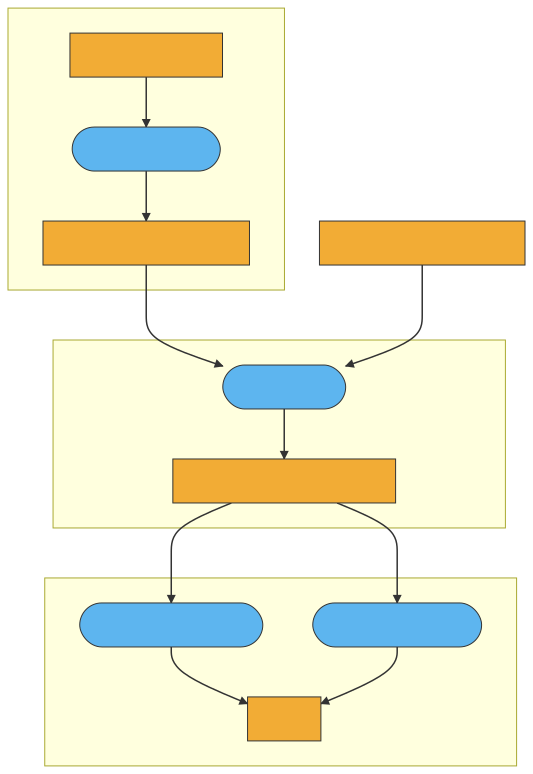
\includegraphics[width=0.6\textwidth]{figures/process}
%  \caption{Experimental setup, orange = data, blue = process}
%  \label{fig:process}
%\end{figure}




% 1.2 Compression Approach
\section{Compression Approach}\label{sec:compression-approach}
XXX MEAN AND AVG DIFFERENCES are used by logistic regression model.
XXX What is the uncertainty interval used here?
The first approach, introduced in PAN2020 and based on \cite{teahan2003compression}, uses a text compression method to determine the chance that two texts were written by the same author.
The compression of a text can be seen as encoding said text with a given encoding.
Thus, as discussed in \cite{brown1992upperBoundEntropy}, text compression can be used to estimate an upper bound to the entropy, i.e. the amount of information of characters in English text.
More specific, by using the compression model of some text A, the cross-entropy of encoding a text B with this model can be calculated.
This approach uses the Prediction by Partial Matching (PPM) model, a standard model for lossless text compression, first introduced by \cite{cleary1984PPM}.
During training, for each pair, the PPM of the first text is used to encode the second text and vice-versa.
In this process, the cross-entropy of the first to the second text can be calculated and vice-versa.
In other words, if the compression of one text with the compression model of the second text works well, the chance that both are written by the same author can be considered high.
The source code used is based on a reimplementation of the Authorship Attribution approach from \cite{teahan2003compression} as part of a reproducibility study in \cite{potthast2016reimplementation}.
An adaption for Authorship Verification stems from PAN20\footnote{\url{https://github.com/pan-webis-de/pan-code/tree/master/clef20/authorship-verification}}.
The source code extending the algorithm to use phonetic features is available on GitHub\footnote{\url{https://github.com/torond/teahan03-phonetic}}.
% Add figure, only showing cross-validation side!

% 1.3 Unmasking Approach
\section{Unmasking Approach}\label{sec:unmasking-approach}
XXX What is the uncertainty interval used here?
% Intro: Embedding in context of related work (at the time), more complex but now baseline
% Invented by Koppel & Schler, cite paper
Unmasking was first introduced by \cite{koppel2004unmasking} in 2004.
% Main idea 1-2 sentences: Why is it called Unmasking? feature removal -> degradation
In short, it exploits the degradation of classifier accuracy when removing distinguishing features.
It turns out that removing those features iteratively leads to a faster degradation on text pairs by one author than on those by different authors.
Thus, the algorithm "unmasks" the text pairs and thereby reveals the information needed for classification.\\

% Formal definiton & explanation: unmasking step
This approach comprises two steps: First, a cross-validation method is employed to create the accuracy degradation curves for all training samples.
Secondly, a meta-classifier is trained on the resulting curves to differentiate between same-author and different-author curves.\\
For a given pair, the texts are seen to be created by two generative processes $p_1$ and $p_2$.
To compute a curve for a pair, both texts are chunked into parts longer then 500 words without splitting paragraphs.
The 250 words with highest average frequencies in the two texts are used as features.
\textcolor{violet}{TBD: Note bag-of-words approach}
In a 10-fold cross-validation linear SVM models are trained to classify if a chunk belongs to $p_1$ or $p_2$.
The resulting accuracy is noted and the three most influential positive and negative features are removed from the feature set \textcolor{teal}{(Is influential the right word here?)}.
The cross-validation and feature removal are repeated until there are no features left.\\
% meta-learning step
The set of curves is then used to train a meta-classifier linear SVM model.
\textcolor{teal}{Note: Rearrange the following sentences to only cite \cite{bevendorff2019unmaskingShortTexts} once.}
As brought to the point by \cite{bevendorff2019unmaskingShortTexts}, features used are "the curve points, the curves' point-wise first- and second-order derivatives, and the derivatives sorted by steepest point-wise drop" \textcolor{teal}{(Should this be paraphrased rather then quoted?)}.\\
% Adaptation for short texts by Bevendorff et al., how is this different? Which features are actually being used?
Unmasking is one of the most robust Authorship Verification algorithms \textcolor{teal}{(\cite{bevendorff2019unmaskingShortTexts})}.
But as it requires sufficient chunks of no less than 500 words length, it is only applicable for book-length texts.
To counter this, \cite{bevendorff2019unmaskingShortTexts} generalizes the algorithm to accommodate for short texts.
Chunks are generated by oversampling the bag-of-words pool of a given text.
Words from this pool are picked randomly without replacement until a length of 700 words is reached and the pool is reset afterwards.
In total, 30 chunks are generated, which are then used for curve generation as above, with the only exception that the five most positive and negative features are removed instead of only three.
As this approach introduces a significant amount of variance in the resulting curves, the unmasking step is repeated three times and the curves are averaged.
This time, the meta-classifier uses the curves' "central-difference gradients (first- and second-order), as well as their gradients sorted by magnitude" \textcolor{teal}{(\cite{bevendorff2019unmaskingShortTexts})}.
\cite{bevendorff2019unmaskingShortTexts} also supplies an implementation of the generalized unmasking algorithm which is used as the basis for our research\footnote{\url{https://github.com/webis-de/unmasking}}.\\
\textcolor{violet}{TBD: Explain that we'll use transcriptions with bag-of-words first, then $Dolgo$ with n-grams.}
%We conduct two experiments using the unmasking algorithm.
%First, we simply used phonetic transcriptions of text pairs as the input to the unmasking algorithm.
%Secondly, we use the features $features_{clever}$ (change notation) instead of the averagely most frequent words.
Note that we only use the Gutenberg dataset for unmasking, as processing the fanfiction dataset would for each of the transcriptions would take multiple weeks.
%We suspect that the differences would not be significant. (Can I phrase that like this??)
We added an out-of-fold cross-validation functionality to the unmasking framework to extract as much information as possible from the much smaller Gutenberg dataset.
The results are then compared to results obtained from verbatim text.
%(Maybe add more code details! What else was added etc.)

%Notes (Koppel and Schler 2004):
%AV as described in the paper is Authorship Attribution -> Goes on to reformulate: AV's question is whether a pair of text sets were created by the same process (author) or different processes.
%-> How does this extend to sets when there's more than 1 author in the "investigated" set?
%-> It sounds like the set of same-author texts must have one author.
%-> Also in paper we have 2 sets of texts, in PAN AV we have a list of pairs. Is this the same?
%Determines "depth of difference" between two sets of texts

%\section{Methods using supra-segmental features}
%% Time Series Modelling in the Analysis of Homeric Verse, Pawłowski 2010
%Manual annotation of long / short syllables and stress / no-stress syllables (p.86).
%ARIMA method for time series modelling.\\
%Rhythmical series are easier to model -> goodness of fit ~ rhythmicity
%
%
%"All the suprasegmental features are characterized by the fact that they must be described in relation to other items in the same utterance.
%It is the relative values of pitch, length, or degree of stress of an item that are significant.
%... The absolute values are never linguistically important.
%But they do, of course, convey information about the speaker's age, sex, emotional state, and attitude toward the topic under discussion."\cite{ladefoged2014courseInPhonetics}

% http://udel.edu/~dlarsen/ling101/slides/Suprasegmentalshandout.pdf
% english has non-distinctive length differences.
% p.15 In English, stress is sometime non-predictable, sometimes predictable.
\chapter{Results}\label{results}
% Introduction: PAN20 uses these measures, so we do, too.
For the evaluation of our approaches we use several traditional as well as recently proposed measures.
\textcolor{olive}{(textbook citation needed for following definitions)} We use the convention that a pair is in the positive class iff both texts are written by the same author.
$tp$, $tn$, $fp$, $fn$ stand for the number of cases that where classified correctly as positive (true positives), correctly as negative (true negatives), falsely as positive (false positives) and falsely as negative (false negatives) respectively.\\
% Explain OOF cross-validation
% Precision
The \textbf{precision} $pre = \frac{tp}{tp+fp}$ of a classifier is the percentage of correct positive classifications $tp$ over all classifications $tp+fp$.
Thus, a precision approaching 1 indicates that an AV classifier's same-author predictions are near fully correct, meaning that there are nearly no false positives.\\
% Recall
The \textbf{recall} $rec = \frac{tp}{tp+fn}$ of a classifier is the percentage of correctly classified positive samples $tp$ over all positive samples $tp+fn$.
The lower the recall, the fewer same-author cases are recognized and predicted as such by an AV classifier.
In turn, a recall of 1 indicates that all same-author cases have been correctly identified.\\
% F1
Ideally, we want a system that classifies all same-author cases and only those as positive.
To measure this behavior, the \textbf{F1-score} $F_1 = 2\cdot\frac{prec\cdot{}rec}{prec+rec}$ can be used.
If both, precision and recall, approach 1 the F1-score of an AV classifier also approaches its maximum of 1.
Note that the F1 score weights precision and recall equally.
Especially for forensic Authorship Verification applications though, a high precision is more important than a high recall, as same-author decisions might be used as evidence and therefore must be reliable.
Also, in our setup, the F1 score ignores true negatives and therefore does not give an insight into how well the classifier detects different-author cases correctly.
For this, the different-author class would need to be assigned the positive label.\\
To mitigate some of the problems of the measures above and to better asses AV classifier performance, we use two more recently introduced measures.
% C@1, Point: non-answers (0.5) are possible
To measure include same-author and different-author classifications in the evaluation, one could use the accuracy $acc = \frac{tp+tn}{n}$, where $n = tp+tn+fp+fn$ is the total number of cases.
However, as \cite{bevendorff2019unmaskingShortTexts} points out, the results are often uncertain.
Also, in real-world applications wrong answers might be worse than non-answers.
Therefore, to give classification systems the option to withhold answers for difficult-to-decide cases, we use the \textbf{c@1-score} introduced by \cite{penas2011c_at_1} and adopted by PAN.
It is defined as $c@1 = \frac{n_{ac}}{n}+\frac{n_{ac}}{n}\cdot{}\frac{n_u}{n} = \frac{1}{n}\cdot{}\left(n_{ac}+\frac{n_{ac}}{n}\cdot{}n_u\right)$ where $n$ is again the total number of cases, $n_{ac} = tp+tn$ is the number of accurately classified cases and $n_u$ is the number of undecided cases.
This way, undecided cases count towards the c@1-score as if they were answered with the accuracy of the decided cases.
When an AV classifier gives an answer to all cases, the C@1-score is reduced to the accuracy.
A system that leaves all cases unanswered, receives a score of 0.\\
% F0.5u
Lastly, we use the \textbf{F0.5u-score} introduced by \cite{bevendorff2019unmaskingShortTexts}.
It is defined as $F_{0.5u} = \frac{(1+0.5^2)\cdot{}n_{tp}}{(1+0.5^2)\cdot{}n_{tp}+0.5^2\cdot{}(n_{fn}+n_u)+n_{fp}}$.
As mentioned above, a high precision result is more robust than a high recall one.
To account for this, the F0.5u-score weights precision two times as much as recall.
In addition, it also allows the classifiers to give non-answers.
However, as unanswered cases are often not useful in real-world applications, it interprets them as wrong answers.
Thus, the F0.5u-score highly emphasizes on the precision of an AV classifier.\\

% PAN20 measures:     AUC, C@1, F0.5u, F1, overall
% Unmasking measures: Precision, Recall, C@1, F0.5u


The results of our experiments can be seen in figures \ref{tab:p_unmasking_gb}, \ref{tab:p_teahan_ff} and \ref{tab:p_teahan_gb}.
The tables show the absolute values of the transcription systems and their statistical significance compared to verbatim text in the first row.
The thresholds for statistical significance are:
\begin{itemize}
    \item $*$: statistically significant ($p < 0.05$)
    \item $*\! *$: very statistically significant ($p < 0.01$)
    \item $*\! *\! *$: highly statistically significant ($p < 0.001$)
\end{itemize}
$+$ marks an increase and $-$ marks a decrease compared to the top row.
For example, $0.5936^{*\! *}_{-}$ indicates very statistically significant decrease of the current transcription's performance compared to verbatim text.


% First: Unmasking
% ->
%- For GB Unmasking: Argue 32 runs for stable results. This still only creates 262 curves. Show which parameters where used for those 32 runs
% - still variance is high, needs about 9%? to be significant
Before analyzing the final results, let us take a look at the sets of the degradation curves that resulted from Unmasking
% 4 gram curves fall much quicker! Show them! -> Rather run again with better window.
% As tehere are no non-answers, f05u is only precision-enhanced, and c@1 prob also has changes

% Then: Teahan Compression
Increasing this interval improves precision and recall, because $non$-$answers$ are omitted in their calculation and thus only those answers are counted that the classifier is more certain of.
On the other hand, $F0.5u$ deteriorates as it counts $non$-$answers$ as wrong classifications.
Decreasing the uncertainty interval leads to a general decrease in performance as uncertain answers are counted  (they are binarized).

% FF
%As cleaning step is phonetically informed we'll use verbatimorignal for comparing.

%For r values higher than 0.05, prec rec higher, f05u cat1 lower.
%Throwing out cases, prec rec f1 only consider cases where classifier is more sure about the result.


% GB
%For CV, CV 4-grams, and Dolgo 4-grams the dataset is too small and all samples are predicted to be false, thus, Precision and Recall are ill-defined (zero division) and we'll leave these out.
%Removed because ill-defined: 'cv', 'cv_4grams', 'dolgo_4grams', 'punct_4grams', 'dolgo', 'asjp_4grams', 'refsoundex', 'soundex'

% Also: Remember to answer the questions from the Introduction


% Compare to other approaches from PAN20
%As indicated earlier, through cross validation, we can use the entire data set for training and for testing, thus milking it in the most effective way. hehe, correction lolol.
% Note Gutenberg dataset is really small


In the following, we will discuss a number of possible reasons for the overall negative trend that phonetic transcriptions bring to the results.\\
Converting graphemes to phonemes, in our case verbatim text to its $IPA$ transcription, is a difficult task.
Moreover, when transcribing automatically, the transcription algorithm does not have any information about the pronunciation of the speaker of a given text.
Thus, usually text is transcribed to either the General (North) American pronunciation or the Received Pronunciation\footnote{British English}.
We use g2pE by \cite{kyubyong2019g2pE} which employs the Carnegie Mellon University Pronouncing Dictionary to look up transcriptions for words.
The CMU dictionary uses North American English as its pronunciation standard.
Thus, by transcribing we assume that the author has a North American English phonetic preference.
Transcribing, for example, both an Irish author's and a Nigerian author's texts to American English, one can imagine that a lot of phonetically relevant information, that could be used to distinguish them, is lost.
In the same vein, authors might \textit{actively} make efforts to impart certain phonetic qualities into their texts that are based on topic rather than the author's unconscious phonetic preference.
This becomes especially clear when an author uses direct speech, which often occurs in the datasets we use as they are both based on sets of fictional stories.
The ``voice in the author's head'' when writing a direct speech passage presumably varies greatly depending on the traits of the character depicted in the story.
Thus, extracting these features might aid in topic or genre identification more so than in Authorship Verification.
To mitigate this, direct speech could be removed from text entirely.\\
Another limitation of phonetic transcriptions for Authorship Analysis is due to the low-level nature they work at.
An authors' freedom of self-expression is limited on the sub-segmental level, i.e., concerning individual sounds.
Usually, the meaning of a word changes together with its pronunciation.
The only words for which this is not the case are synonyms such as the words "begin" and "start".
Thus, authors that want to express similar ideas arguably will sound similar on the sub-segmental level not because of their phonetic preference but due to the proximity of the topics.
More importantly, if authors want to express different ideas the resulting transcriptions will also be different, without the Authorship Verification classifier knowing if this difference stems from two unique authors with varied phonetic preferences or from one author discussing different topics.
Supra-segmental features such as stress or prose can be utilized more freely and might give a more informative base for Authorship Analysis.\\
Lastly and perhaps most importantly, standard Unmasking without using $n$-grams works on the lexical level, i.e., it uses entire words as atomic units and ignores the information encoded by the symbols inside a word.
With the step of transcription, however, we are precisely attempting to enhance this inner-word information.
Thus, for Unmasking the transcription of data serves only as a phonetically-informed binning method for types.
To mitigate this, we tried to use an $n$-gram based transcription method, with XXX results.\\



Describe n-gram effects of pt!


% Problem 3 / Following thoughts: Phonetic transcriptions / features are probably bad Authorship predictors but better predictors for other features such as genre, topic, age of setting.
\begin{table}
\caption{Significance of changes for Unmasking using the Gutenberg dataset, bonferroni-corrected.}
\label{tab:p_unmasking_gb}
\centering\small
\begin{tabular}{@{}l@{\hspace{1\tabcolsep}}lllll@{}} % Use @{\hspace{2\tabcolsep}} to double the spacing
\toprule
\bf System & \bf Precision & \bf Recall & \bf F1 & \bf F0.5u & \bf c@1 \\
\midrule
$Verbatim$ & $0.7545$ & $0.6539$ & $0.6977$ & $0.6784$ & $0.6875$ \\
\midrule
$IPA$ & $0.7537$ & $0.6701$ & $0.7004$ & $0.6641$ & $0.6833$ \\
$ASJP$ & $0.7284$ & $0.667$ & $0.6893$ & $0.6455$ & $0.676$ \\
$Dolgo$ & $0.7551$ & $0.6733$ & $0.7046$ & $0.6617$ & $0.6792$ \\
$RefSoundex$ & $0.7297$ & $0.6275$ & $0.6673$ & $0.6233^{*\! *}_{-}$ & $0.6542$ \\
$Metaphone$ & $0.7193$ & $0.6028$ & $0.648^{*}_{-}$ & $0.6143^{*\! *}_{-}$ & $0.6423^{*\! *}_{-}$ \\
$Soundex$ & $0.7333$ & $0.6363$ & $0.6677$ & $0.6234^{*\! *}_{-}$ & $0.6512$ \\
$CV$ & $0.6316^{*\! *}_{-}$ & $0.5757$ & $0.5936^{*\! *}_{-}$ & $0.5171^{*\! *\! *}_{-}$ & $0.5381^{*\! *\! *}_{-}$ \\
$IPA$ $4$-$grams$ & $0.6536^{*\! *}_{-}$ & $0.5814$ & $0.6043^{*\! *}_{-}$ & $0.5505^{*\! *\! *}_{-}$ & $0.5976^{*\! *\! *}_{-}$ \\
$ASJP$ $4$-$grams$ & $0.721$ & $0.6148$ & $0.6553$ & $0.6086$ & $0.6257$ \\
$P$ $4$-$grams$ & $0.718$ & $0.6339$ & $0.6658$ & $0.6207^{*}_{-}$ & $0.6387^{*}_{-}$ \\
$Dolgo$ $4$-$grams$ & $0.6894$ & $0.5964$ & $0.6245$ & $0.5558^{*\! *\! *}_{-}$ & $0.6012^{*\! *}_{-}$ \\
$CV$ $4$-$grams$ & $0.6161^{*\! *}_{-}$ & $0.5853$ & $0.5926^{*\! *}_{-}$ & $0.4868^{*\! *\! *}_{-}$ & $0.5151^{*\! *\! *}_{-}$ \\
$P$ & $0.7155$ & $0.6672$ & $0.6859$ & $0.6452$ & $0.6745$ \\
$PL$ & $0.7707$ & $0.6801$ & $0.7153$ & $0.6876$ & $0.7079$ \\
$PLS$ & $0.7676$ & $0.6614$ & $0.7031$ & $0.6572$ & $0.6905$ \\
\bottomrule
\end{tabular}
\end{table}

\begin{table}
\caption{Significance of changes for the compression approach using the Fan-fiction dataset compared to verbatim text (uncleaned), $r=0.05$, bonferroni-corrected.}
\label{tab:p_teahan_ff}
\centering\small
\begin{tabular}{@{}l@{\hspace{1\tabcolsep}}lllll@{}} % Use @{\hspace{2\tabcolsep}} to double the spacing
\toprule
\bf System & \bf Precision & \bf Recall & \bf F1 & \bf F0.5u & \bf c@1 \\
\midrule
$Verbatim$ $(orig.)$ & $0.7635$ & $0.8092$ & $0.7856$ & $0.714$ & $0.7431$ \\
\midrule
$IPA$ & $0.7532^{*\! *\! *}_{-}$ & $0.7846^{*\! *\! *}_{-}$ & $0.7686^{*\! *\! *}_{-}$ & $0.7098^{*\! *\! *}_{-}$ & $0.7291^{*\! *\! *}_{-}$ \\
$Verbatim$ & $0.7604^{*\! *\! *}_{-}$ & $0.8078^{*\! *}_{-}$ & $0.7833^{*\! *\! *}_{-}$ & $0.7101^{*\! *\! *}_{-}$ & $0.739^{*\! *\! *}_{-}$ \\
$ASJP$ & $0.7602^{*\! *}_{-}$ & $0.7857^{*\! *\! *}_{-}$ & $0.7727^{*\! *\! *}_{-}$ & $0.7148$ & $0.7353^{*\! *\! *}_{-}$ \\
$Dolgo$ & $0.7474^{*\! *\! *}_{-}$ & $0.7757^{*\! *\! *}_{-}$ & $0.7612^{*\! *\! *}_{-}$ & $0.6992^{*\! *\! *}_{-}$ & $0.7174^{*\! *\! *}_{-}$ \\
$RefSoundex$ & $0.7564^{*\! *\! *}_{-}$ & $0.7811^{*\! *\! *}_{-}$ & $0.7685^{*\! *\! *}_{-}$ & $0.7049^{*\! *\! *}_{-}$ & $0.7259^{*\! *\! *}_{-}$ \\
$Metaphone$ & $0.772^{*\! *\! *}_{+}$ & $0.7907^{*\! *\! *}_{-}$ & $0.7813^{*\! *\! *}_{-}$ & $0.7266^{*\! *\! *}_{+}$ & $0.7477^{*\! *\! *}_{+}$ \\
$Soundex$ & $0.7129^{*\! *\! *}_{-}$ & $0.7717^{*\! *\! *}_{-}$ & $0.7411^{*\! *\! *}_{-}$ & $0.6758^{*\! *\! *}_{-}$ & $0.6839^{*\! *\! *}_{-}$ \\
$CV$ & $0.6371^{*\! *\! *}_{-}$ & $0.8172^{*\! *}_{+}$ & $0.716^{*\! *\! *}_{-}$ & $0.6253^{*\! *\! *}_{-}$ & $0.5842^{*\! *\! *}_{-}$ \\
$P$ & $0.7528^{*\! *\! *}_{-}$ & $0.7914^{*\! *\! *}_{-}$ & $0.7716^{*\! *\! *}_{-}$ & $0.7092^{*\! *\! *}_{-}$ & $0.7304^{*\! *\! *}_{-}$ \\
$PL$ & $0.7228^{*\! *\! *}_{-}$ & $0.7868^{*\! *\! *}_{-}$ & $0.7534^{*\! *\! *}_{-}$ & $0.6782^{*\! *\! *}_{-}$ & $0.6949^{*\! *\! *}_{-}$ \\
$PLS$ & $0.6994^{*\! *\! *}_{-}$ & $0.7773^{*\! *\! *}_{-}$ & $0.7363^{*\! *\! *}_{-}$ & $0.6604^{*\! *\! *}_{-}$ & $0.668^{*\! *\! *}_{-}$ \\
\bottomrule
\end{tabular}
\end{table}


\begin{table}
\caption{Significance of changes for the compression approach using the Gutenberg dataset compared to verbatim text, $r=0.05$, bonferroni-corrected.}
\label{tab:p_teahan_gb}
\centering\small
\begin{tabular}{@{}l@{\hspace{1\tabcolsep}}lllll@{}} % Use @{\hspace{2\tabcolsep}} to double the spacing
\toprule
\bf System & \bf Precision & \bf Recall & \bf F1 & \bf F0.5u & \bf c@1 \\
\midrule
$Verbatim$ & $0.871$ & $0.7354$ & $0.7909$ & $0.6163$ & $0.645$ \\
\midrule
$IPA$ & $0.8545$ & $0.676^{*}_{-}$ & $0.7383^{*}_{-}$ & $0.5951$ & $0.5396^{*\! *\! *}_{-}$ \\
$ASJP$ & $0.8738$ & $0.7241$ & $0.7786$ & $0.607$ & $0.5325^{*\! *\! *}_{-}$ \\
$Metaphone$ & $0.9441^{*\! *}_{+}$ & $0.7265$ & $0.8005$ & $0.5824^{*\! *}_{-}$ & $0.4088^{*\! *\! *}_{-}$ \\
$IPA$ $4$-$grams$ & $0.9117$ & $0.74$ & $0.7895$ & $0.5611^{*\! *\! *}_{-}$ & $0.3793^{*\! *\! *}_{-}$ \\
$P$ & $0.8816$ & $0.7178$ & $0.7801$ & $0.5979$ & $0.5655^{*\! *\! *}_{-}$ \\
$PL$ & $0.8664$ & $0.7237$ & $0.7734$ & $0.592^{*\! *}_{-}$ & $0.5554^{*\! *\! *}_{-}$ \\
$PLS$ & $0.8006$ & $0.7056$ & $0.737^{*}_{-}$ & $0.6165$ & $0.6197$ \\
\bottomrule
\end{tabular}
\end{table}
\chapter{Conclusion}\label{conclusion}
% Short summary
In this paper we analyzed the viability of phonetically transcribing textual data prior to the use in Authorship Verification algorithms.
Despite our initial expectations, we conclude that using phonetic transcriptions of data for Unmasking by \cite{koppel2004unmasking} and the compression approach by \cite{teahan2003compression} does \textit{not} result in an improvement in performance.
In fact, we observed many statistically significant decreases in overall performance.
Nonetheless, we could identify a trend, namely the more a phonetic transcription system decreases the vocabulary size after transcription, the worse the performance of the algorithms.
This may indicate that broader transcription systems lose more information that could have been useful for classification.
The other extreme, inflating the vocabulary to 3.5 times its original size by generating $4$-grams of the already detailed \textit{IPA} transcription, also leads to a very significant drop in performance across most of the measures analyzed.
The only exception to this is the \textit{Metaphone} algorithm in conjunction with the compression approach when using a sufficiently sized dataset, in our case one of the datasets introduced in \cite{bevendorff2020overview} comprising more than 50,000 training samples.
For this configuration, we could record a slight improvement of 0.85\% in precision over using verbatim text.\\
As is naturally the case with negative results, we cannot disprove that phonetically informed methods are generally not viable for Authorship Verification.
We did, however, discuss some possible explanations for the absence of positive results from our research:
\begin{itemize}
    \item During automatic transcription, too much phonetic information may be lost, as the transcription algorithm does not have any information about the specific pronunciation of the author.
    \item When working on the level of individual sounds, as we do with phonetic transcriptions, the sounds expressed when verbalizing an idea are often tied to their meaning. Therefore, sub-segmental features might be better predictors for topic than for authorship.
    \item Unmasking works on the lexical level, because it treats words as atomic units and ignores the information encoded inside of them. This way, phonetic transcriptions are reduced to simple data reduction methods not exhausting their full potential.
\end{itemize}
Regarding possible improvements of our research, a more thorough inspection of the observed trend of diminishing performance with decreasing transcription granularity could lead to the substantiation of a correlation thereof.
If other non-phonetically-informed token binning methods exhibit a similar correlation between performance and granularity, one could conclude that this trend is, in fact, not due to any phonetic phenomena.
A different way of verifying this would be to down-sample the transcriptions so the vocabulary sizes are the same.
Any remaining differences in performance cannot stem from the systems' granularities.\\
To achieve a better understanding of the utilization of phonetic transcriptions, verbatim and phonetically transcribed texts could be combined and feature selection algorithms could be used to identify the subset of features that is being employed by the algorithms in classification.
This way, it could be determined whether AV classifiers utilize phonetically transcribed data over verbatim data.\\
Additionally to the investigations above, a detailed grid search for the best parameters for each transcription could be performed and might lead to an improvement of the results.\\
For further research, we suggest a more profound investigation of the existence and nature of the \textit{phonetic preference}.
With a more thorough understanding of the ways people are influenced by their personal and subconscious phonetic palette, more meaningful feature extraction methods could be developed.
These could include more in-depth approaches that, for example, disambiguate semantic information by analyzing certain punctuation structures within the text on the phonetic level.
Also, shifting the focus from the low-level sub-segmental features to supra-segmental features spanning longer segments of text, such as stress, intonation, and rhythm, seems promising as authors have more freedom of self-expression on this level.

% Structure
% 0. Abstract
% 1. Introduction
% 2. Basics (What is phonetics, transcriptions)
% 3. Related Work
% 4. Experiments
%   4.1 Sub-segmental
%   4.2 Supra-segmental
% 5. Results / Analysis / Discussion
% 6. Conclusion / Outlook

% Bibliography
\bibliographystyle{plainnat} % requires package natbib. An alternative is apalike
\bibliography{literature}    % load file literature.bib

\end{document}

